%! Author = borisdeletic
%! Date = 06/05/2023

% Preamble
\documentclass[11pt]{article}

% Document
\begin{document}

\appendix
\section{Constrained HMC Parameter Values}\label{sec:param_table}
    The below table shows the values used for all input parameters into CHMC as defined in the paper.

    \begin{center}
    \begin{tabular}{|l|c|r|}  % Alignment for each cell: l=left, c=center, r=right, | indicates vertical line
        \hline  % Horizontal line
        Symbol & Description & Value \\
        \hline
        $\epsilon_0$  & Initial step size   & 0.1   \\
        $L$  & Path Length   & 100   \\
        $\delta$  & Target Acceptance Rate   & 0.8   \\
        $\gamma$  & Adaption scaling  & 0.05  \\
        $\kappa$  & Adaption shrinkage  & 0.75  \\
        $\mu$  & Asymptotic Target & -1  \\
        \hline
    \end{tabular}
    \end{center}
    These parameters were selected based on those used in the paper~\cite{hoffman2011nouturn} and manual tweaking.

\section{Code Implementation}\label{sec:code_implementation}
    The code was implemented in C++ and optimised for speed and modularity.
    We use an object-oriented interface design based on \emph{dependency injection}.
    This allows the code base to be easily compartmentalised and extended by other authors, while also keeping an easy
    plug-in design for any likelihood function.

    \begin{figure}[h!]
        \center
        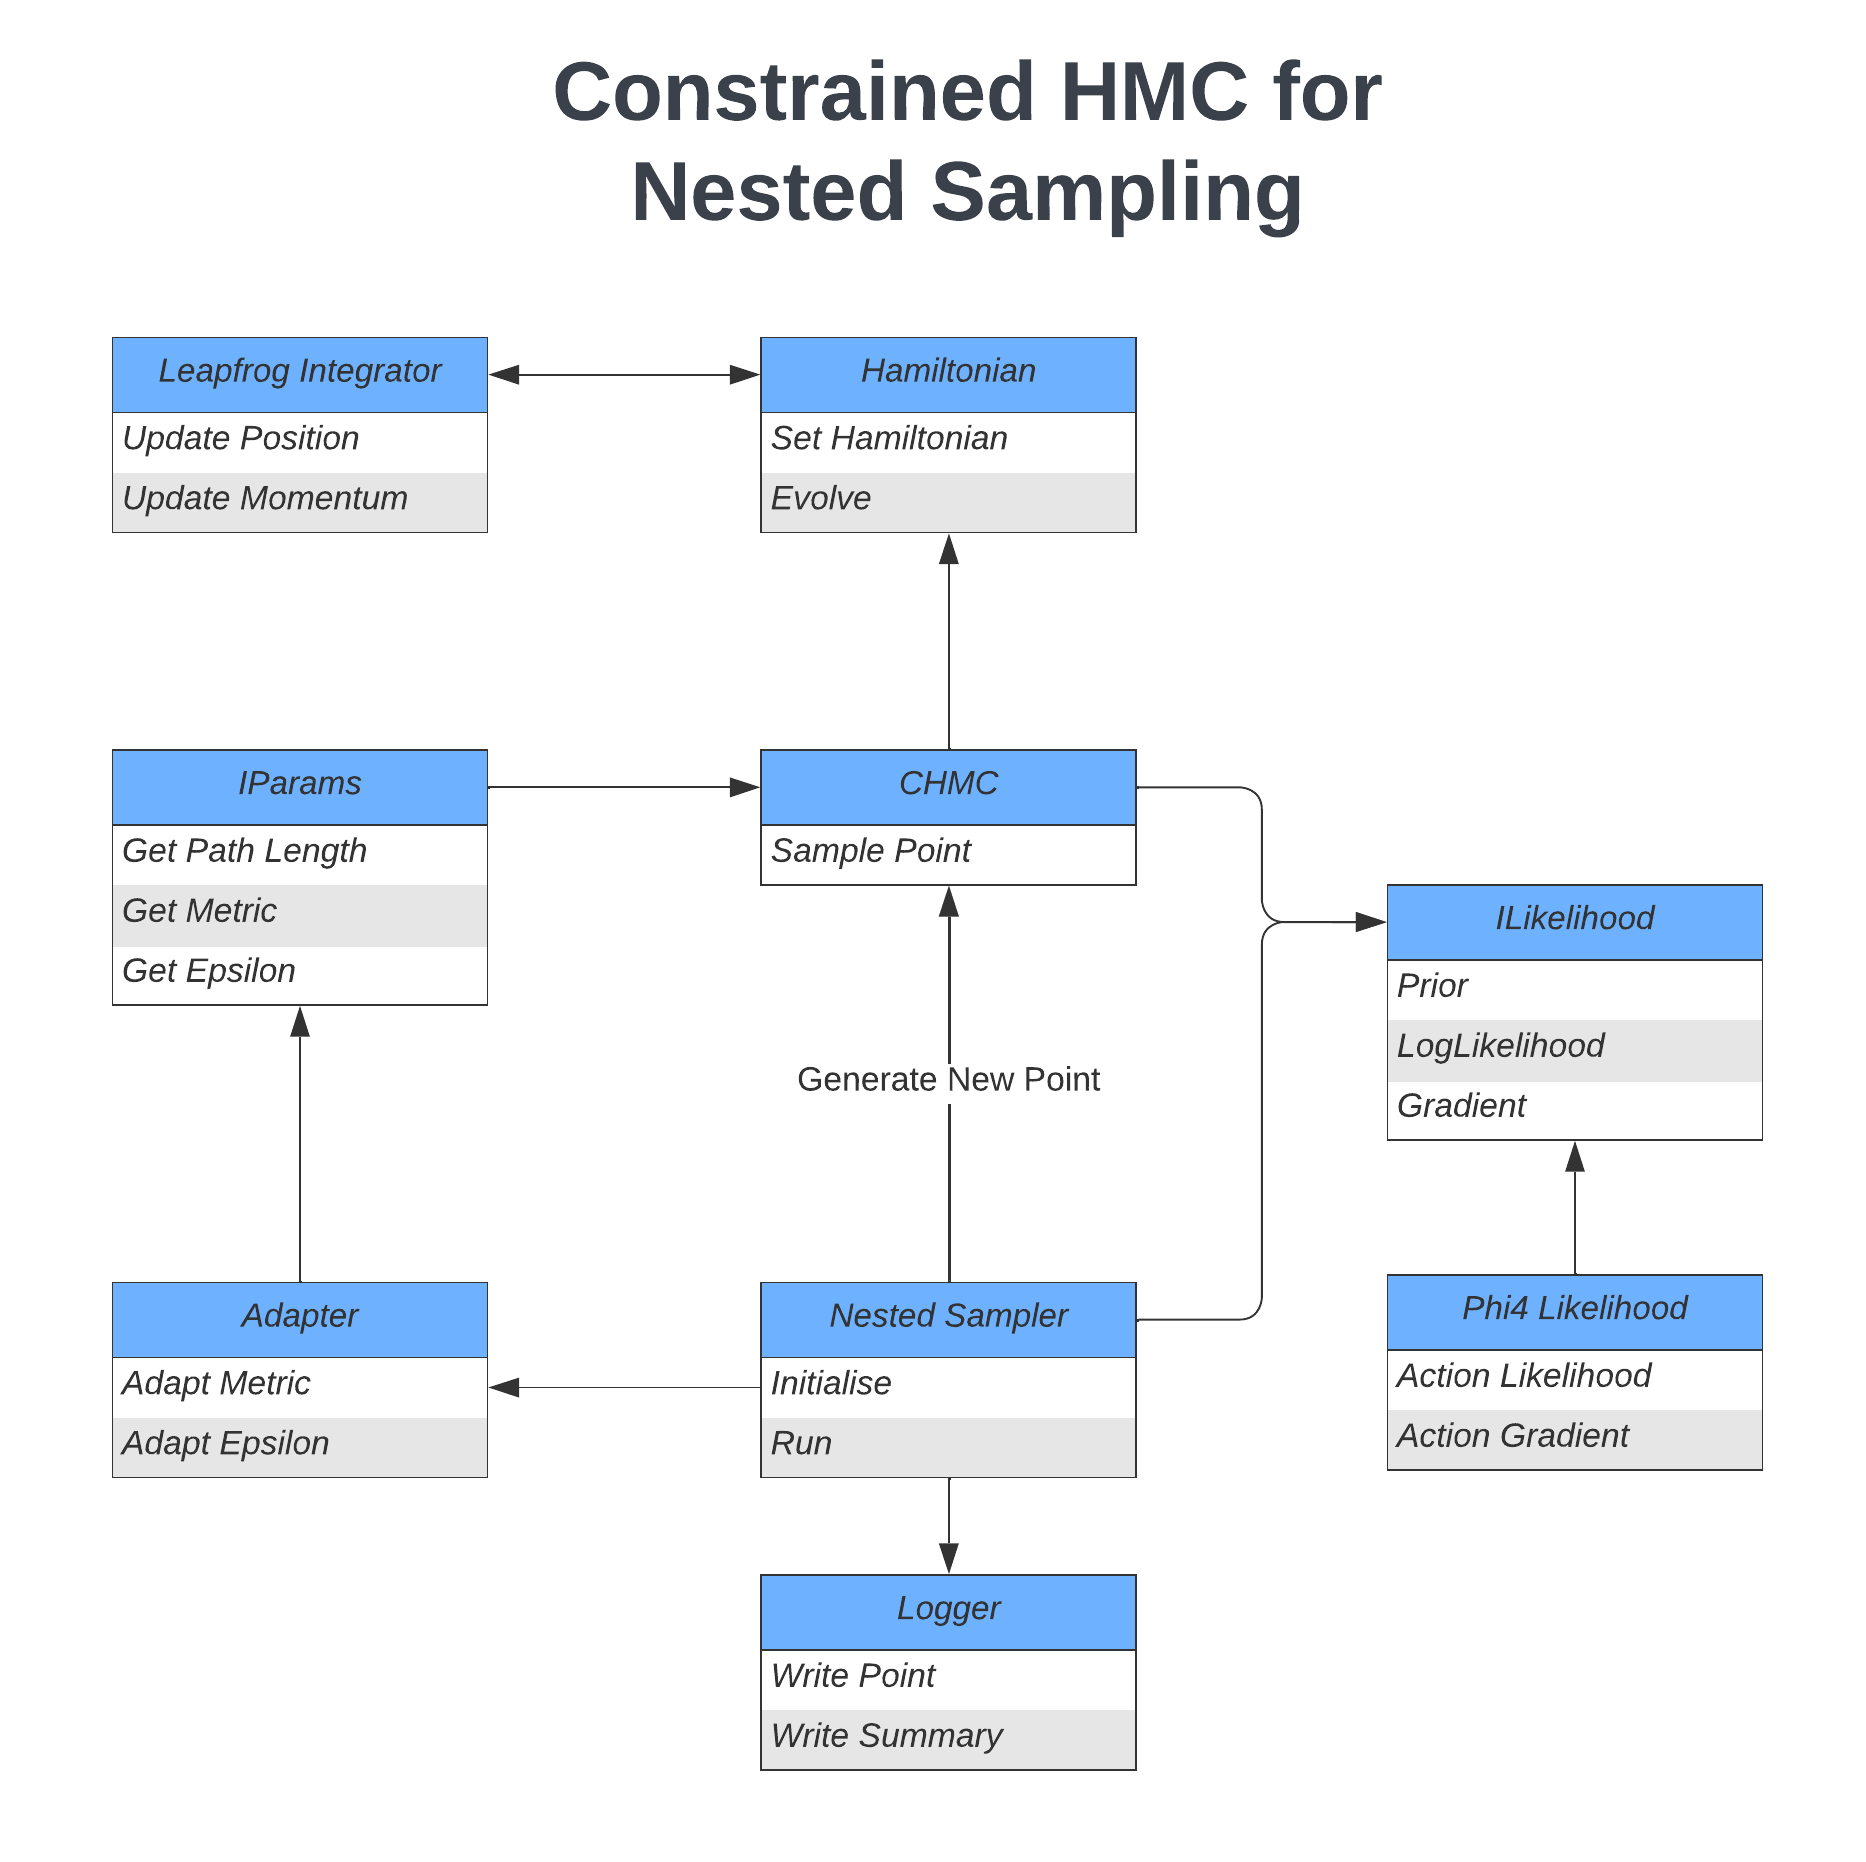
\includegraphics[width=\linewidth]{../figures/UML_Diagram}
        \caption{
            UML Diagram illustrating the relationship between each objects.
            Each class was implemented as an independent code base hiding implementation details, then injected into
            each other to expose the desired functions.
            An interface design is used for the likelihood class, so the program does not require any specific knowledge
            of the likelihood.
            This allows one to simply implement the desired likelihood, such as $\phi^4$ theory, without making any
            additional modifications.
        }\label{fig:uml_diagram}
    \end{figure}

    The \textsc{Eigen3} library was used for heavy all calculations, which is an optimised scientific
    linear algebra library.

    To ensure correctness, we implemented a set of unit tests using the \textsc{GoogleTest} framework to rigorously
    check the functionality of each class.

\section{Auto Differentiation}\label{sec:autodiff}
    Auto differentiation is a modern approach to numerically calculating gradients with no numerical
    error~\cite{carpenter2015stan}.
    The essential idea is that a compiler can break down a program to its base operations and automatically apply the
    chain-rule repeatedly to calculate its gradient.
    Recent advancements in machine learning have greatly increased the demand for auto differentiation tools and now
    highly optimised frameworks exist to calculate gradients for any code base.

    One such example is \textsc{Enzyme}~\cite{NEURIPS2020_9332c513, 10.1145/3458817.3476165, 10.5555/3571885.3571964},
    a tool that takes arbitrary existing code base in a variety of languages (including C++) and computes the
    gradient of that function.
    We demonstrate this capability on the Rosenbrock function which allows CHMC to automatically run without needing to
    specify any gradients.

    The D-dimensional Rosenbrock function is defined as
    \begin{equation}\label{eq:rosenbrock}
        f(\theta) = AD + \sum_{i=0}^D\left(\theta_i^2 - A \cos (2 \pi \theta_i) \right)
    \end{equation}

    In code block below, we show how to use \textsc{Enzyme} to automatically calculate the gradient
    of the Rosenbrock function.

    \begin{widetext}
    \begin{lstlisting}[label={lst:enzyme}]
    //Rosenbrock Likelihood
    double Likelihood::likelihood(double* theta, int size, double A) {
        double f = A * size;
        for (int i = 0; i < size; i++) {
            f += pow(theta[i], 2) - A * cos(2 * M_PI * theta[i]);
        }
        return f;
    }

    \\ Rosenbrock Autogradient
    int enzyme_dup, enzyme_const;
    extern double __enzyme_autodiff(...);
    double Likelihood::gradient(double* theta, double* d_theta, int size, double A) {
        return __enzyme_autodiff(likelihood,
                                 enzyme_dup, theta, d_theta,
                                 enzyme_const, size, A);
    }
    \end{lstlisting}
    \end{widetext}

    The result in~\cref{fig:rosenbrock} shows the function contours and auto gradient, demonstrating how auto
    differentiation is a viable solution for CHMC with no numerical rounding error.
    \begin{figure}[h!]
        \center
        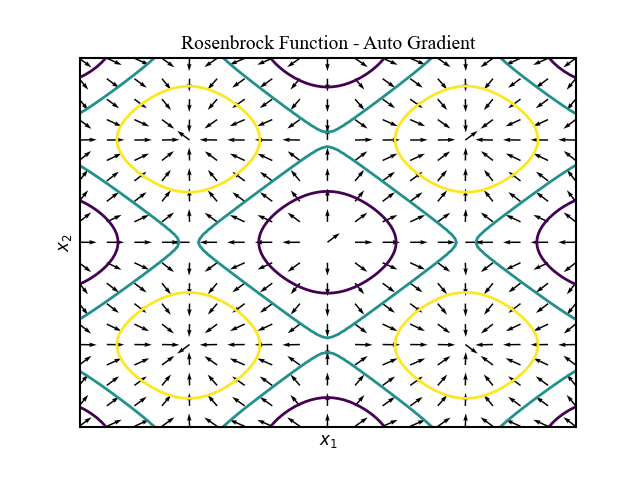
\includegraphics[width=\linewidth]{../figures/RosenbrockAutodiff}
        \caption{
            Rosenbrock function~\eqref{eq:rosenbrock} and automatic differentiation gradient field plot.
            We demonstrate the validity of auto differentiation as a viable solution for any CHMC likelihood function.
        }\label{fig:rosenbrock}
    \end{figure}


\section{Metric Adaption with the Equipartition Theorem}\label{sec:metric_derivation}
    Consider a $D$ dimensional Hamiltonian with kinetic and potential energy
    \begin{equation}\label{eq:hamiltonian_appendix}
    H = \frac{1}{2} \mathbf{p}^T M^{-1} \mathbf{p} + U,
    \end{equation}
    with momentum distributed as $\mathbf{p} \sim \mathcal{N}(0, \sigma=M)$.
    For simplicity, we use a scaled unit metric $M = \alpha \mathbb{1}$.
    According to the equipartition theorem, the energy is equally shared among the degrees of freedom.
    Therefore, we match the variance in potential energy per dimension to the kinetic energy.
    \begin{equation}\label{eq:var_matching}
    \begin{aligned}
        \frac{1}{D} \mathrm{Var}[U] &= \mathrm{Var}[T]  \\
        \mathrm{Var}[U] &= D\mathrm{Var}\left[\frac{1}{2} \mathbf{p}^T M^{-1} \mathbf{p}\right]  \\
        \mathrm{Var}[U] &= \frac{D}{4 \alpha^2} \mathrm{Var}\left[\mathbf{p}^T \mathbf{p}\right] \\
        \mathrm{Var}[U] &= \frac{D}{4 \alpha^2} \mathrm{Var}\left[\sum_i^D{\mathbf{p}_i^2}\right] \\
        \mathrm{Var}[U] &= \frac{D^2}{4 \alpha^2} \alpha^4 \\
        \mathrm{Var}[U] &= \frac{D^2 \alpha^2}{4} \\
        \alpha = \frac{2}{D} \sqrt{\mathrm{Var}[U]}
    \end{aligned}
    \end{equation}
    Which gives the result for the metric
    \begin{equation}\label{eq:metric_adaption_appendix}
    M = \frac{2}{D} \sqrt{\mathrm{Var}[U]} \mathbb{1},
    \end{equation}


\end{document}